\documentclass{tufte-handout}

%\geometry{showframe}% for debugging purposes -- displays the margins

\usepackage[T1]{fontenc}
\usepackage{newpxtext}
\usepackage{amsmath}
\usepackage{mweights}
\usepackage{microtype}

% Set up the images/graphics package
\usepackage{graphicx}
\setkeys{Gin}{width=\linewidth,totalheight=\textheight,keepaspectratio}
\graphicspath{{graphics/}}

\title{Overview of the Digestive System}
\author{Olivia S. Anderson and Dave Bridges}
\date{}  % if the \date{} command is left out, the current date will be used

% The following package makes prettier tables.  We're all about the bling!
\usepackage{booktabs}

% The units package provides nice, non-stacked fractions and better spacing
% for units.
\usepackage{units}

% The fancyvrb package lets us customize the formatting of verbatim
% environments.  We use a slightly smaller font.
\usepackage{fancyvrb}
\fvset{fontsize=\normalsize}

% Small sections of multiple columns
\usepackage{multicol}

% Provides paragraphs of dummy text
\usepackage{lipsum}

% These commands are used to pretty-print LaTeX commands
\newcommand{\doccmd}[1]{\texttt{\textbackslash#1}}% command name -- adds backslash automatically
\newcommand{\docopt}[1]{\ensuremath{\langle}\textrm{\textit{#1}}\ensuremath{\rangle}}% optional command argument
\newcommand{\docarg}[1]{\textrm{\textit{#1}}}% (required) command argument
\newenvironment{docspec}{\begin{quote}\noindent}{\end{quote}}% command specification environment
\newcommand{\docenv}[1]{\textsf{#1}}% environment name
\newcommand{\docpkg}[1]{\texttt{#1}}% package name
\newcommand{\doccls}[1]{\texttt{#1}}% document class name
\newcommand{\docclsopt}[1]{\texttt{#1}}% document class option name

\begin{document}

\maketitle% this prints the handout title, author, and date

\begin{abstract}
\noindent This lecture will provide an overview of the anatomy and physiology of the digestive tract. Food is digested to release its contained nutrients in order to be absorbed into the body for cellular use. To understand how human bodies utilize macronutrients, it is important to have a clear
comprehension of how (macro-) nutrients from food are digested and subsequently absorbed from the digestive tract to circulation (i.e., how do
macronutrients get into our bodies). 
\end{abstract}

\tableofcontents

\pagebreak
\section{Learning Objectives}

\begin{itemize}
\item Identify the organs that make up the digestive tract
\item Describe the structural components of the digestive tract organs
\item Explain how digestive processes are regulated
\item Describe key features of the main organs in the digestive tract
\item Understand the roles of digestive secretions from accessory organs on the breakdown of macronutrients
\item Identify the unique features of the small intestine and illustrate how they enhance digestion and absorption
\item Describe how digested macronutrients are absorbed across thesmall intestine
\item Explain the fate of inadequately digested materials
\item Examine health conditions related to the digestive tract

\end{itemize}

\section{Key Vocabulary and Concepts}

\begin{itemize}
\item Alimentary canal
\item Bolus and chyme
\item Duodenum, jejunum, and ileum
\item Gastrin, Secretin, Ghrelin and CCK
\item Glands, including lingual and salivary
\item Gut associated lymphoid tissue (GALT)
\item Enteric nervous system 
\item Enterohepatic circulation and bile
\item Esophageal sphincters (upper and lower)
\item Lumen
\item Mucuosa, Submucosa, Muscularis externa and Serosa
\item Plexus of Meissner and Plexus of Auerbach
\item Sympathetic and parasympathetic nervous system
\item Villi, microvilli and brush border

\end{itemize}

\section{The Digestive Tract Organs}

The alimentary canal, the \textbf{main organs} that make up the digestive tract, is a continuous, hollow tube. The alimentary canal consists offive main organs (oral cavity, esophagus, stomach, small intestine, large intestine). Each specific organ has unique features to aid in the digestion process. A specific type of muscle called a sphincter connects each consecutive main organ. Sphincters act as a passageway for the digested food product. When food material is not present in the tract, the sphincters constrict closing off the passageways. When food material is present and moving down the tract, a regulatory signal results in the \emph{relaxation} of the sphincter muscle, opening the passageway and allowing the food material to travel down the tract from one organ to the next. 

\begin{marginfigure}
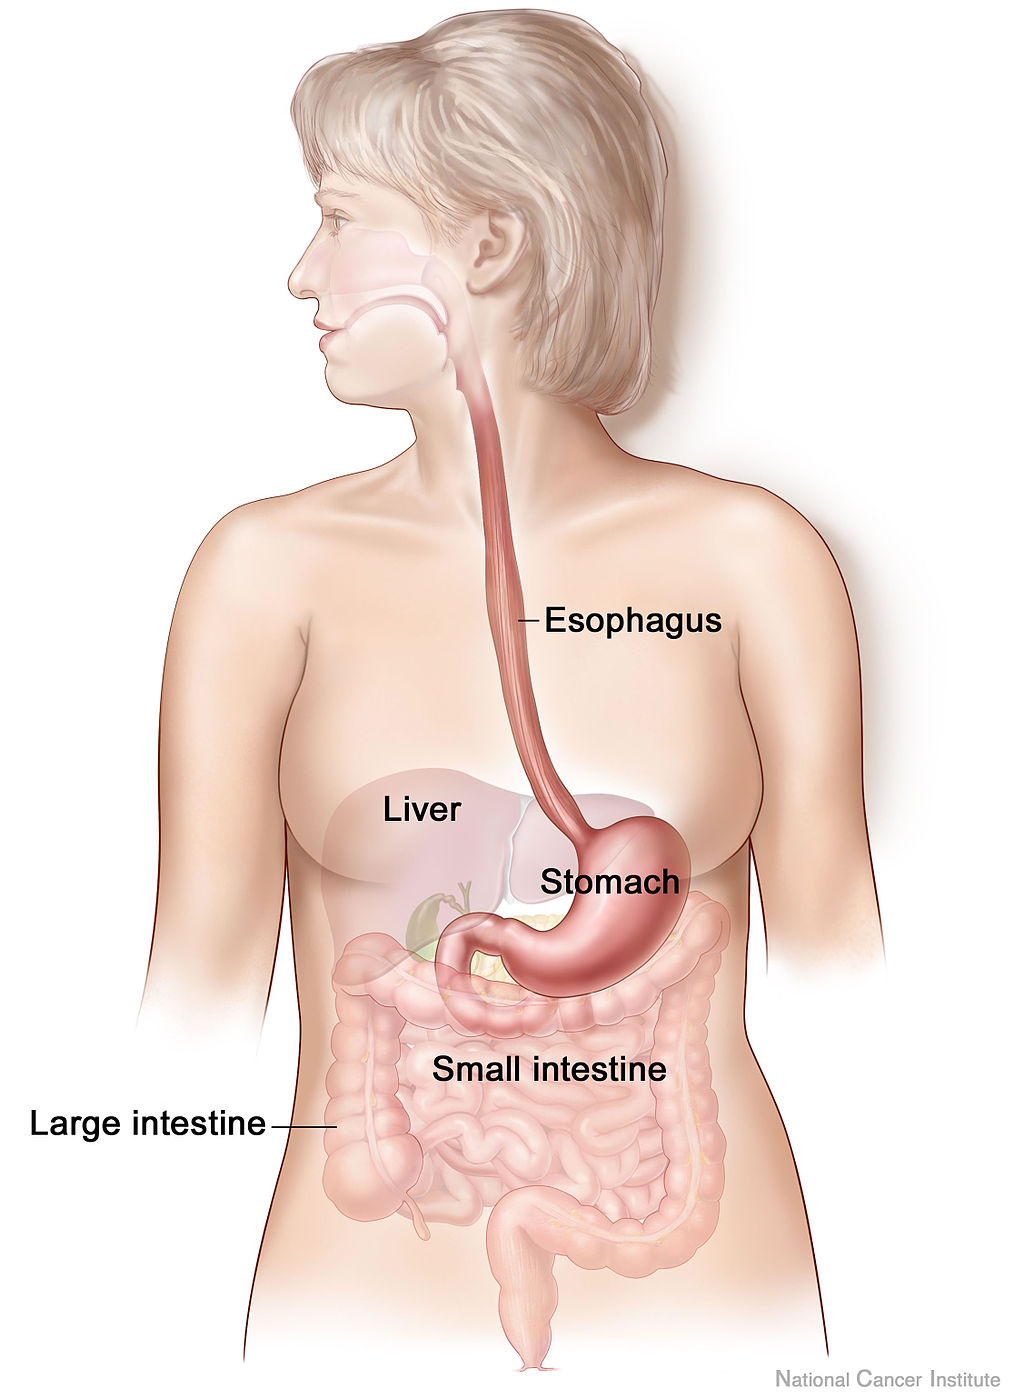
\includegraphics{figures/digestive-tract.jpg}
\caption{Diagram of the main organs of the digestive tract.  From National Cancer Institute \url{http://visualsonline.cancer.gov/details.cfm?imageid=3925}.}
\end{marginfigure}

The digestive tract also consists of organs referred to as \textbf{accessory organs} (salivary glands, pancreas, liver, gallbladder). Their main role in digestion is to provide, store and deliver secretions to the main organs for digestion and mobilization of food material. Although accessory organs are not in direct contact with the food material as it travels down the tract, the proper functioning of accessory organs is crucial for proper digestive processes. 

\section{Structure of the Digestive Tract}

Remember that the main organs of the digestive tract form a continuous, hollow tube. The hollow space, where the digested food material travels is called the \emph{lumen}. The main organs are made up of four distinct layers (see ~\ref{tab:layers}). Each of the four layers has their own unique functions that support proper digestion. The innermost layer is called the mucosa and in itself has three sublayers --- the epithelial lining, lamina propria and muscularis mucosa. The epithelial lining is comprised of exocrine and endocrine cells. The exocrine cells' main function is to secrete mucus to lubricate the food material. The endocrine cells secrete hormones into the bloodstream that signal for digestive processes to occur. The second sublayer is the lamina propria. This sublayer of the mucosa contains tissue called \emph{gut associated lymphoid tissue (GALT)}. GALT plays an important immune function in the body by releasing macrophages and lymphocytes that ward off foreign microorganisms that humans ingest. The last sublayer is the muscularis mucosa. This is a thin smooth muscle layer that produces twitch-like movements when it contracts. The main purpose of the twitching is to disengage food material that may have gotten stuck on the digestive tract wall.

\begin{margintable}
\caption{Layers of the digestive tract.}\label{tab:layers}
\begin{tabular}{ll}
\textbf{Layer} & \textbf{Sublayer} \\
Mucosa & Epithelia \\
       & Lamina Propria \\
       & Muscularis Mucosa \\
Submucosa &  \\
       & Plexus of Meissner \\
Muscularis Externa & =Circular Muscle \\
         & Plexus of Auerbach \\
       & Longitudinal Muscle \\    
Serosa & \\             
\end{tabular}
\end{margintable}

\newthought{The second layer is the \emph{submucosa}}, which is made of blood vessels, elastic fibers and a bundle of nerves. As food is ingested and moves down the tract, the digestive organs can stretch (think of the stomach), the elastic fibers help to expand the organs, but also to get them back to their original size and shape. The submucosa contains a nerve bundle called the \emph{Plexus of Meissner} that plays a role in regulating secretions from accessory organs into the main organs and in controlling blood flow (see more in Regulation of Digestive Processes section). The third layer is the muscularis externa made of inner-circular and outer-longitudinal muscles. These muscles work together to produce a muscle movement called peristalsis. Peristalsis is a wave-like contraction that pushes food material forward through the tract. There is another nerve bundle located in the muscularis externa called the \emph{Plexus of Auerbach}. This Plexus plays a role in controlling muscle movements. 

The outermost layer is the \emph{serosa}. The main functioning of the serosa is to provide structural support for the tract and to secrete lubricant to help protect the inner wall of the digestive tract.

\section{Regulation of Digestive Processes}
As food material is digested, the tract itself is highly regulated to ensure nutrients are properly digested to the correct molecular form that is suitable for absorption and that digestion occurs in a timely manner (not too fast, not too slow). The digestive tract has two main types of regulation, including neural and hormonal. The neural regulation stems from the peripheral nervous system and includes both sympathetic and parasympathetic control, thus you can think of the regulation from each to have opposite effects. The sympathetic slows digestion while the parasympathetic stimulates digestion.\marginnote{\textbf{Reflection:} From the information we have discussed thus far, what could be one example of what the sympathetic nervous system might induce? And the same consideration for the parasympathetic?} 

\newthought{Extrinsic and intrinsic nerves make up the sympathetic and parasympathetic nervous system of the digestive tract}. The extrinsic nerves that connect the digestive tract to the spinal cord and brain control the constriction and relaxation of the muscles within the digestive tract as well as play a role in secretion of substances into the tract from the accessory organs. The parasympathetic extrinsic nerve endings that penetrate the digestive tract release acetylcholine resulting in the promotion of digestion, or in other words, increased muscle movements and secretions. The sympathetic extrinsic nerve endings in the digestive tract secrete norepinephrine stimulating decreased secretions and muscle movement and constriction. This muscle control is important for the passage of food material from one consecutive main organ to the next. The intrinsic nerves include fibers innervating the interior of the digestive tract, and they control digestive secretions (Plexus of Meissner) and peristalsis (Plexus of Auerbach). The intrinsic nerves are often referred to as a nervous system specific to digestive control and are collectively called the \emph{enteric nervous system} (ENS).  For more details see \citet{Furness2012}.

The central nervous system also plays a role in activating digestion. External sensory stimuli such as thought, smell, and taste of food can trigger the release of gastric juice (the production and composition of gastric juice is described below in Stomach subsection) which stimulates digestion in the stomach. The endocrine cells of the mucosal layer of the tract release hormones that help control digestive processes in addition to the neural control. The  list of hormones found to play a role in digestive regulation is exhaustive. For the purposes of this discussion, we only focus on a select four that have been well characterized in their role for digestion (Table~\ref{tab:gi-hormones}). 

\begin{margintable}
\caption{Sites of production of key digestive hormones}\label{tab:gi-hormones}
\begin{tabular}{ll}
\textbf{Hormone} & \textbf{Site of Production} \\
Gastrin          & Stomach                     \\
Secretin         & Small Intestine             \\
CCK              & Small Intestine             \\
Ghrelin          & Stomach                    
\end{tabular}
\end{margintable}

\newthought{Gastrin} is produced by the stomach (and to a lesser degree in the small intestine) in response to the stomach distending as well as the presence of macronutrients within the lumen of the stomach. It plays a role in stimulating motility and digestive secretions locally. Gastrin also stimulates the emptying of the food material from the stomach to the next main organ, the small intestine. As part of its function, gastrin stimulates hydrochloric acid (HCl) release within the stomach. Increasing HCl initiates the inactivation of gastrin. 

\newthought{Secretin is produced in the small intestine and released in response to the acidic food materials entering the small intestine}. Secretin slows down the rate of gastric emptying and gastric digestive secretions. In turn, secretin initiates the release of digestive juices from the pancreas, which is important for digestion within the small intestine. 

\newthought{Cholecystokinin (CCK) is also produced in the small intestine.} It stimulates the release of a substance called bile that is important for fat digestion and mobilization within the tract. It also stimulates the release of enzymes produced in the pancreas important for catalyzing digestion processes within the small intestine.

\newthought{Ghrelin is a hormone that is secreted in the absence of food}. It stimulates hunger and has been found to initiate the production of gastric juices in the anticipation of food intake \citep{Inui2004}. Increasing research explores other hormones like Ghrelin that play a role in satiety signaling pathways. For further reading, \citet{Schwartz2000} provide a nice overview of these satiety signals and how targeting these pathways is a potential treatment strategy for weight control.\marginnote{\textbf{Reflection:} In general, describe how malfunctioning of the pancreas could
affect digestion?}

\section{The Main Organs and Their Functions}
Again, the digestive tract consists of five main organs. The organs are categorized as the  \emph{upper digestive tract} (oral cavity, esophagus and stomach) and the \emph{lower tract} (small and large intestine). In this section we will discuss the main macronutrient digestion events that occur within each
organ.

\subsection{Oral Cavity}\index{Oral Cavity}
The oral cavity is the first main organ food comes into contact with. The oral cavity encompasses the mouth and the pharynx. The features of the mouth that assist initial digestion include teeth, salivary glands\sidenote{\textbf{Definition:} Glands --- small organs throughout the body with the
main function of secreting substances to other parts of the body.} and the tongue. The digestion of food can be \emph{mechanical} as well as \emph{chemical} (\textit{i.e.}, enzymatic). Before moving forward, it is important to distinguish between mechanical and chemical breakdown of food. Mechanical digestion is simply breaking down larger food particles to smaller ones without the occurrence of a chemical reaction (\textit{e.g.}, hydrolysis). Mechanical digestion can occur by sheer forces, like the teeth, or by rigorous muscle movements, like peristalsis. Chemical digestion occurs when the food nutrients come into contact with an enzyme or acid and undergo a chemical reaction (likely hydrolysis) forming a simpler nutrient that will eventually be broken down into its absorbable form. 

The teeth in the oral cavity start digestion by the mechanical breakdown of food fibers.\ \emph{Salivary glands} in the mouth secrete a substance called saliva. Saliva is compromised mostly of water as well as key components that help with digestion and immunity. Salivary alpha amylase\sidenote{You can tell this is an enzyme since it ends in \emph{-ase}, and it primarily functions to breakdown amylose a sugar we will talk about in a few lectures}, released with saliva, is the first enzyme that begins chemical breakdown via hydrolysis of carbohydrates within the mouth. Mucus is also found in saliva, which helps lubricate the food for ease of travel through the tract. One last component of saliva is \emph{lysozyme}. This is an enzyme that attacks foreign bacteria found in food products. This is especially important for oral health, like tooth decay. The tongue combines the food and saliva for chemical digestion and lubrication to occur. Once the food is well mixed with saliva, the food mass is called a \emph{bolus}. Another key purpose of the tongue is to help push the bolus to the back of the mouth to initiate swallowing so the movement of the bolus continues down the tract for further digestion. Another set of glands located on the tongue is called \emph{lingual glands}. These produce an enzyme called \emph{lingual lipase} that is incorporated into saliva. Lingual lipase plays a role in the digestion of certain types of lipids. Lingual lipase travels with the bolus but remains inactive until it reaches the stomach.

\subsection{Esophagus}\index{Esophagus}
If you imagine swallowing a piece of food (technically a bolus), it is initially a voluntary action. It is a conscious effort to chew and get the bolus to the back of the mouth to the pharynx. Following the act of swallowing the digestive process becomes involuntary because of neural and hormonal regulation, as described above. As the bolus moves from the pharynx of the oral cavity, the first sphincter called, accordingly, the \emph{upper esophageal sphincter} (UES) relaxes, thus opening up a passageway for the bolus to enter the esophagus. At the same time as the UES opens, a flap of cartilage called the epiglottis shifts to block the trachea (part of the respiratory tract). The blockage of the trachea prevents food from entering the lungs, which could potentially be life threatening (see Conditions of Interest section below). The bolus travels down the digestive tract by peristalsis. The force of peristalsis is quite strong (have you ever successfully ate or drank something while standing on your head?). Altogether the bolus is in the esophagus for no more than a few seconds. As the bolus approaches the bottom of the esophagus, the \emph{lower esophageal sphincter} (LES) relaxes and the bolus enters the stomach. As we will discuss later, following the relaxation of the UES and LES, the constriction of the UES and LES are of great importance so the bolus does not have the ability to travel back to organs it has already been in but rather continue down the lumen of the alimentary canal to continue proper digestion. 

\subsection{Stomach}\index{Gastric Juice}\index{Stomach}
The bolus is now in the stomach. At rest the adult stomach is about 1.5 ounces. The stomach has some unique features on the mucosal layer. The mucosa has structural pits along the entirety of it. These gastric pits contain glands with four different cell types. Each cell type secretes certain substances that aid in motility and chemical digestion (Table~\ref{tab:gi-cells}). The secretions from the mucous neck, parietal\index{Parietal Cells}, chief\index{Chief Cells} and endocrine cells\index{Enteroendocrine Cells} make up gastric juice. The mucus in the gastric juice acts as a lubricant to the bolus. Hydrochloric acid (HCl)\index{Hydrocholoric Acid} decreases the pH of the stomach environment. The lower pH from HCl acts as an immune defense to kill off foreign microorganisms and activates enzymes that are also part of gastric juice such as pepsinogen. In addition to pepsinogen, lipase is another enzyme that is part of gastric juice. These enzymes target protein and lipids, respectively. Two additional enzymes originating from the mouth are also present in the stomach including salivary alpha amylase\index{Digestive Enzymes!Salivary Alpha Amylase} and lingual lipase. Salivary alpha amylase has traveled with the bolus from the oral cavity to the stomach. Alpha amylase thrives in a more neutral environment so it is inactivated anywhere from a few minutes to a half hour after entering the stomach \citep{Rohleder2009}. Lingual lipase becomes activated in the acidic environment. The bolus is mixed with gastric juice by a churning movement from the oblique muscles of the muscularis externa\index{Muscularis Externa}. Once sufficiently mixed with gastric juice the bolus is now called the \emph{chyme}.\index{Chyme} 

\begin{margintable}
\caption{Gastric cell types and their secretions}\label{tab:gi-cells}
\begin{tabular}{ll}
\textbf{Cell Type} & \textbf{Secretion} \\
Mucous neck	 & Mucus                     \\
Parietal & HCl             \\
Chief & Pepsinogen, lipases, water \\
Endocrine & Regulatory hormones                    
\end{tabular}
\end{margintable}

\newthought{There are several points of regulation of digestion activity in the stomach.} First, the thought, smell, and taste of food can send a signal to the central nervous system that simulates the production and release of gastric juice. There is hormonal control by gastrin\index{Hormones!Gastrin}, produced by endocrine cells in the gastric pits. Gastrin will function to release gastric juice from the pits. It will also promote the gastric motility of chyme to continue to move forward through the alimentary canal. Thus, in the stomach, gastrin is promoting digestive processes. Another hormonal point of regulation is by secretin. Secretin\index{Hormones!Secretin} is produced by the small intestine. As the chyme is emptied from the stomach to the small intestine (i.e., gastric emptying), secretin will signal the gastric cells to decrease the production of components for gastric juice and the motility in the stomach to slow. Overall, although secretin is produced in the small intestine, it plays a role in regulating digestion processes in the stomach.\ \marginnote{\textbf{Reflection:} What was something you learned as you read about the upper portion of the digestive tract?}

\subsection{Small Intestine}\index{Small Intestine|(}
The chyme is emptied into the small intestine as the pyloric sphincter relaxes. The small intestine itself is made of three distinct sections, the \emph{duodenum, jejunum, and ileum}. Anatomically-speaking the duodenum is structurally different than the jejunum and ileum whereas the latter two  have no real anatomic distinctions, but as chyme moves down the small intestine, the distinct roles each section has in digestion and absorption of nutrients is clear. The duodenum, being the closest in proximity to the stomach receives the chyme, which is highly acid (pH about 2) from HCl containing gastric juice. The duodenum\index{Small Intestine!Duodenum} contains Brunner's\index{Brunner's Glands} glands that secrete bicarbonate to neutralize the chyme. The jejunum\index{Small Intestine!Jejunum} is where the majority of macronutrient absorption will occur. The ileum\index{Small Intestine!Ileum} is where the minimal absorption of the remaining nutrients (both macro and micro) may occur if they have escaped absorption in the duodenum or jejunum. 

To complete macronutrient digestion, the small intestine provides a means of both mechanical and continued chemical digestion. The muscles of the small intestine contract in a way that results in a back and forth movement called \emph{segmentation}. The purpose of segmentation is two-fold: First, it aids in mechanical breakdown of chyme and Second, it increases the amount of contact time that the nutrients have with the surface of the small intestine, increasing the chance of absorption. Structurally, the small intestine is shaped differently than other areas of the digestive tract. If you were to take a microscopic visual of the lining of the small intestine, it would look like there were finger-like projections shooting in towards the lumen. The finger like projections are called \emph{villi}\index{Villi} and are lined with \emph{enterocytes}\index{Enterocytes} also referred to as intestinal absorptive cells, within the small intestine. The enterocyte has a polarity with an \emph{apical membrane}\sidenote{This is the side facing the digested food, or the lumen of the gastrointestinal tract} and a basolateral membrane\index{Basolateral Membrane}\sidenote{The side in contact with blood or lymph vessels}. If you were to zoom in on one villus you would see that the lining of this finger-like projection contain even smaller finger-like projections called \emph{microvilli}.\ \index{Microvilli}Altogether, the villi and microvilli are referred to as the \emph{brush border}.

\begin{marginfigure}
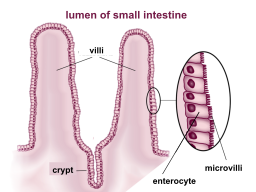
\includegraphics{figures/enterocyte-villi.png}
\caption{Schematic of the relationship between villi, enterocytes and microvilli.  From \url{https://commons.wikimedia.org}.}
\end{marginfigure}

The structure of the brush border allows for a large surface area to permit efficient absorption. The basic absorption pathway of a digested macronutrient in the small intestine would be as follows: lumen $\rightarrow$ across apical membrane of enterocyte $\rightarrow$ through the enterocyte $\rightarrow$ across basolateral membrane of enterocyte $\rightarrow$ capillaries or lymph vessels.\ \index{Apical Membrane}\index{Capillaries}\index{Lymph} 

In addition to a large surface area, the brush border also contains enzymes that catalyze the completion of carbohydrate and protein digestion. Further digestion in the small intestine relies on the pancreas to produce and secrete pancreatic juices. Pancreatic juice contains digestive enzymes that also help complete digestion of carbohydrates, proteins and lipids so they are in a molecular form available for enterocyte transporters allowing for absorption into circulation. The pancreatic juice also contains bicarbonate to neutralize the small intestine environment and maximize digestive enzyme activity. Pancreatic juice is regulated by secretin\index{Hormones!Secretin} and CCK\index{Hormones!CCK}, both of these hormones are produced in the small intestine (Table~\ref{tab:gi-hormones}). 

The liver plays an important role in fat digestion and absorption. The liver is the site for bile synthesis\index{Liver}. Bile is a substance comprised of  cholesterol, bilirubin, water, phospholipids\index{Lipids!Phospholipids} and bile salts. Once produced, the bile is stored in the gallbladder until chyme is present in the small intestine. The bile travels to the duodenum\index{Small Intestine!Duodenum} via the common bile duct. Bile is important first for digestion. The bile salts of bile are amphipathic – the hydrophobic side coalesces to a fat molecule while the hydrophilic side stabilizes the compound in the aqueous environment of the small intestine. As the bile salts are coalesced to the fat molecule, you can think of them as melting the individual lipid droplets apart from each other so digestive enzymes\sidenote{Quick check-in: where are these enzymes coming from again?} have access to them. Once the fat molecules are broken down to their simplest digested form, the bile salts come into play again to help with absorption. This time the bile salts will surround a group of free fatty acids (absorbable form of fats). A group of free fatty acids surrounded by bile salts\index{Bile Salts} are referred to as \emph{micelles}\index{Micelles}. The micelles are stabilized as they reach the enterocytes of the small intestine. Once they reach the brush border membrane, the bile salts are released and the free fatty acids are transported across the enterocyte to the lymph vessels of the villi. Once complete, about 90\% of bile is recycled from the ileum back to the liver through a cycle called \emph{enterohepatic circulation}\index{Enterohepatic Circulation}.\marginnote{\textbf{Reflection:} Which accessory organs play a role in digestion within the small intestine? Explain one role of each accessory organ.}

\newthought{Absorption and transportation of nutrients.} The enterocyte\index{Enterocytes} has the microvilli\index{Microvilli} membrane that project towards the lumen of the tract. This membrane is the apical membrane and thus is the first membrane that the nutrients must cross. Once across the apical membrane the nutrients travel across the enterocyte to the basolateral membrane that is in contact with the blood and lymph vessels\index{Lymph}, thus, the second membrane the nutrients must cross. Macronutrient absorption across the apical and basolateral membranes requires passive diffusion, carrier-mediated transport or pinocytosis depending on what nutrient is being absorbed. The specific type of transportation mechanism will be discussed in the digestion and absorption lectures specific to each macronutrient.\index{Small Intestine|)}

\subsection{Large Intestine}\index{Large Intestine}
The digestive process of macronutrients is not perfect. There will be leftover material that is not properly digested or properly digested material that bypassed the absorption within the small intestine due to lack of contact with the mucosa or unavailable transporters. This material will stimulate the relaxation of the ileocecal sphincter connecting the ileum and the large intestine. Muscle movements keep the material in the proximal region of the large intestine to allow time for absorption of water, sodium and chloride. The undigested carbohydrates and amino acids can serve as fuel for the gut bacteria\index{Gut Microbiome}. As the gut bacteria degrades the carbohydrates and amino acids they release byproducts like short-chain fatty acids (SCFAs). SCFAs\index{Lipids!Short-Chain Fatty Acids} serve a variety of purposes like cellular proliferation, pH alteration, or they can even be absorbed through the enterocytes in the large intestine for utilization of cells in our body (e.g., brain or liver cells). As the undigested material moves down the large intestine water is continually being drawn from it and absorbed into the body. This continuous dehydration results in fecal matter. 

\section{Pathologies Related to GI Structure and Function}

\subsection{Gastroesophageal reflex disease (GERD)}\index{Gastroesophageal Reflex Disease}
Almost everyone has experienced ‘acid reflux' at one point in their life time. This is when gastric juices and/or food materials flow back into the esophagus and sometimes to the mouth. When this happens on a regular basis or over a long period of time it is classified as gastroesophageal reflux disease (GERD). After repeated exposure to acidic contents from the stomach, the mucosal layer of the esophagus can become irritated and inflamed. Over time fibrotic tissue can form resulting in the narrowing of the lumen. If there is repeated exposure in the mouth, this can lead to dental problems such as enamel exposure. 

\newthought{GERD occurs when the LES\index{Lower Esophogeal Sphincter} has not properly closed leaving the passageway from the esophagus to the stomach open.} There are common and well-characterized risk factors that leave the LES in its relaxed state. A large, high-fat meal will remain in your stomach for a longer period of time. The high amount of food eaten will stretch the stomach disallowing the LES to close properly and because the bolus is in the stomach for a longer period of time, there will be increased production of gastric acid. Pregnancy can also lead to GERD because all of the internal organs are more tightly packed due to increased size of the uterus creating an increased pressure on the stomach. During pregnancy there is an increased production of progesterone that is meant to be a muscle relaxer to prepare for delivery. This muscle relaxant affects other muscles in the body including the sphincter muscles. Alcohol and nicotine in cigarettes are muscle relaxants. Spicy and minty foods and chocolate contain compounds within them that cause muscle relaxation. Being overweight is positively associated with GERD.@ 

\newthought{GERD can be treated by identifying the triggers and adapting lifestyle changes to avoid them.} Lifestyle factors that will improve the symptoms of GERD include weight loss\index{Weight loss}, dietary restrictions, cessation of smoking, eating smaller meals and exercise (to lose weight). If lifestyle factors are not working, there are over the counter antacids available. Antacids contain an alkaline like magnesium or calcium that neutralize the stomach environment. Antacids\index{Antacids} are one of the few approved over the counter medications that are safe and acceptable for pregnant women to ingest.

\subsection{Aspiration pneumonia and asphyxiation}\index{Aspiration pneumonia}
Remember that the respiratory tract and digestive tract are separate systems in the body but the organs of the tracts are in close contact to one another. The epiglottis works to block the trachea as the bolus is swallowed. There are certain conditions when these systems do not work in concert with each other resulting in the bolus entering the respiratory tract. This has the ability to occur under conditions of low consciousness or those that affect the swallowing center of the brain. Conditions of low level of consciousness include drug overdose, alcohol poisoning or brain injury. Conditions affecting the swallowing control center in brain include Parkinson's disease, tumor, and stroke. When the bolus enters the trachea a couple things may happen. First, the airway becomes inflamed from irritation from the food, liquids, or even vomit (drug overdose or alcohol poisoning). The inflammation of the airway is referred to as aspiration pneumonitis. If an infection occurs it would become aspiration pneumonia, requiring antibiotic treatment.. In a worst case or unmonitored scenario asphyxiation will occur where an individual would not have sufficient oxygen entering the airways leading to suffocation.  

Patients who are monitored under these conditions require specialized diets where swallowing becomes an easier process on the muscles that are involved. They will likely be prescribed a semi solid (mechanically altered) diet (\textit{e.g.}, peeled fruits, ground meats, noodle consistency, \textit{etc.}). Or in a worst-case scenario, the patient would require enteral or parenteral feeding dependent on the situation. 

\bibliography{library}
\bibliographystyle{plainnat}

\end{document}
